\paragraph{CNN - Convolutional Neural Network}\mbox{}\\

Convolutional neural networks are used to extract intermediate representations of the input. They take advantage of convolutional filters with weights that are learned during training. Such convolutional filters create a convolutional layer. An image passed through a first convolutional layer creates the feature maps. Convolutional layers can be stacked together, creating in the result a convolutional network.
Convolutional layers are usually combined with subsampling techniques, such as pooling. 

\begin{figure}[H]
    \centering
    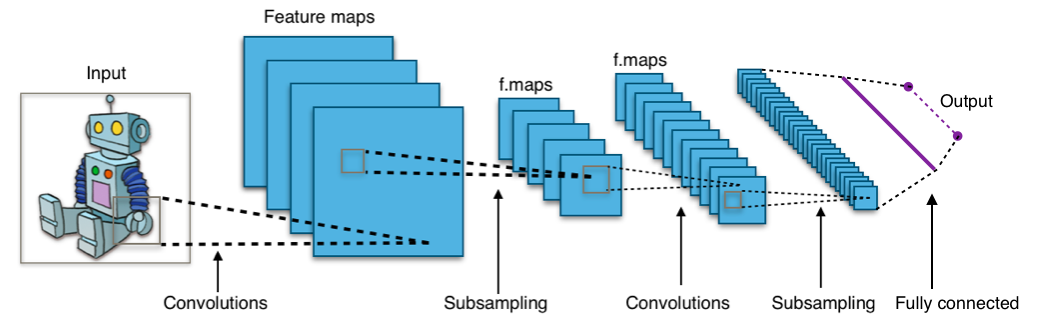
\includegraphics[width=\linewidth]{concept_engineering/Typical_cnn.png}
    \caption{Typical architecture of a convolutional neural network\cite{cnn-typical}.}
    \label{fig:cnn}
\end{figure}


\paragraph{Autoencoder}\mbox{}\\
\begin{figure}[H]
    \centering
    \begin{tikzpicture}[
    box/.style={draw, minimum width=2cm, minimum height=3cm, text width=1.8cm, align=center},
    smallbox/.style={draw, minimum width=1.5cm, minimum height=1.2cm, text width=1.3cm, align=center},
    arrow/.style={->, >=latex, thick},
    label/.style={font=\small}
]

% Components
\node[circle, draw] (input) {Input $x$};
\node[box, right=1cm of input] (encoder) {Encoder};

% Latent space
\node[right=1cm of encoder] (latent) {};
\node[circle, draw, minimum size=1cm, right=0cm of latent] (z) {$z$};

\node[box, right=1cm of z] (decoder) {Decoder};
\node[circle, draw, right=1cm of decoder] (output) {Output $\hat{x}$};

% Reparameterization trick

% Connections
\draw[arrow] (input) -- (encoder);
\draw[arrow] (encoder) -- (z);
\draw[arrow] (z) -- (decoder);
\draw[arrow] (decoder) -- (output);

% Labels
\node[label, below=0.2cm of input] {High-dimensional};
% \node[label, above=0.2cm of mu] {Latent space};
\node[label, below=0.2cm of output] {Reconstructed};

% KL Divergence

% Reconstruction Loss
\draw[<->, >=latex, bend right=30] ($(input.south west)+(1,-0.3)$) to node[below, font=\small] {Reconstruction Loss} ($(output.south east)+(-1.3,-0.2)$);
\end{tikzpicture}
    \caption{Visualization of an autoencoder. Circles are tensors, rectangles neural networks.}
    \label{fig:autoencoder}
\end{figure}
\indent Autoencoder is an architecture of deep learning model that consists of two deep neural networks - Encoder and Decoder. The task of the encoder is to transform the input into latent representation of the input. Usually it compresses it, for example to a vector or smaller matrix/tensor. Decoder then takes such latent representation and transforms it back to its original form. 

The loss function between input $x$ and output $\hat{x}$ is usually one of the following: L1, L2, MSE.

\paragraph{U-Net}\mbox{}\\
\indent U-Net is a special type of convolutional neural network, originally built for the task of image segmentation, especially in medical imaging. Its architecture resembles a U-shape, similar to an autoencoder. The encoder on the left side reduces the input image size while capturing significant features. The right side increases resolution and performs tasks like segmentation, utilizing the features extracted by the encoder via "skip connections." Despite the similarity, U-Net is not considered an autoencoder due to the use of skip connections.

\begin{figure}[H]
    \centering
    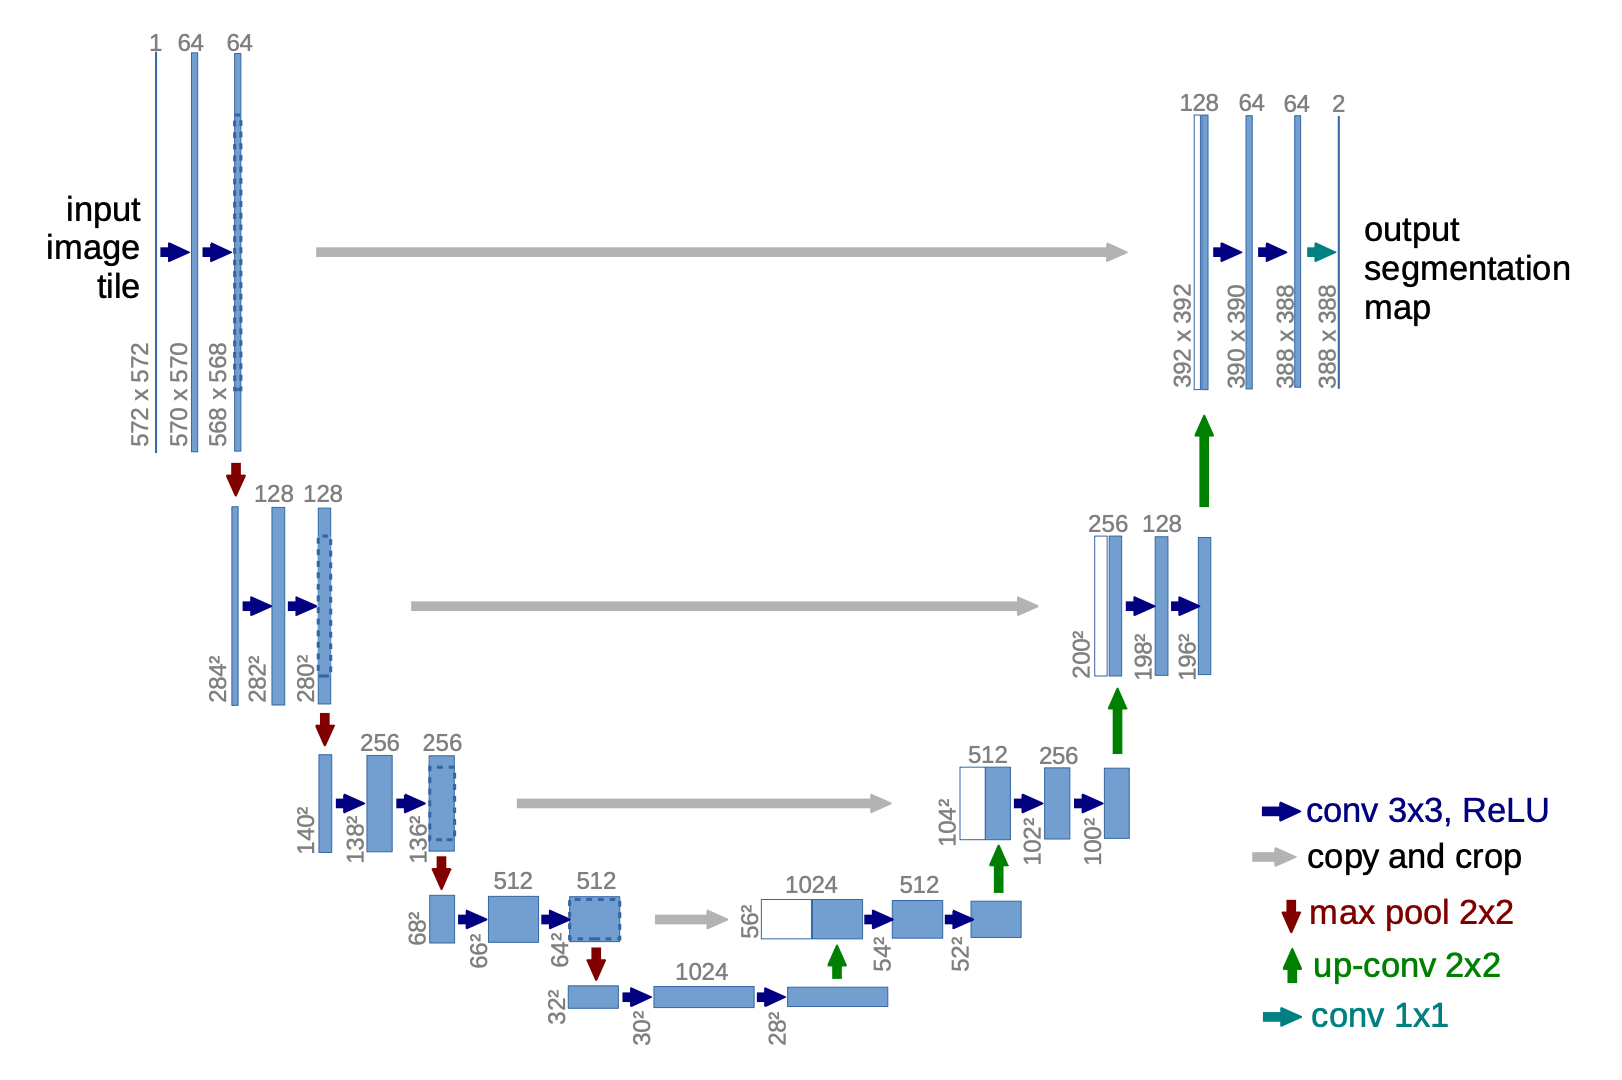
\includegraphics[width=0.9\linewidth]{concept_engineering/unet/U-net.png}
    \caption{U-Net architecture\cite{RFB15a}.}
    \label{fig:unet}
\end{figure}


